%
% ---------------------------------------------------------------
% Copyright (C) 2012-2018 Gang Li
% ---------------------------------------------------------------
%
% This work is the default powerdot-tuliplab style test file and may be
% distributed and/or modified under the conditions of the LaTeX Project Public
% License, either version 1.3 of this license or (at your option) any later
% version. The latest version of this license is in
% http://www.latex-project.org/lppl.txt and version 1.3 or later is part of all
% distributions of LaTeX version 2003/12/01 or later.
%
% This work has the LPPL maintenance status "maintained".
%
% This Current Maintainer of this work is Gang Li.
%
%

\documentclass[
 size=14pt,
 paper=smartboard,  %a4paper, smartboard, screen
 mode=present, 		%present, handout, print
 display=slides, 	% slidesnotes, notes, slides
 style=tuliplab,  	% TULIP Lab style
 pauseslide,
 fleqn,leqno]{powerdot}


\usepackage{cancel}
\usepackage{caption}
\usepackage{stackengine}
\usepackage{smartdiagram}
\usepackage{attrib}
\usepackage{amssymb}
\usepackage{amsmath} 
\usepackage{amsthm} 
\usepackage{mathtools}
\usepackage{rotating}
\usepackage{graphicx}
\usepackage{boxedminipage}
\usepackage{rotate}
\usepackage{calc}
\usepackage[absolute]{textpos}
\usepackage{psfrag,overpic}
\usepackage{fouriernc}
\usepackage{pstricks,pst-3d,pst-grad,pstricks-add,pst-text,pst-node,pst-tree}
\usepackage{moreverb,epsfig,subfigure}
\usepackage{color}
\usepackage{booktabs}
\usepackage{etex}
\usepackage{breqn}
\usepackage{multirow}
\usepackage{natbib}
\usepackage{bibentry}
\usepackage{gitinfo2}
\usepackage{siunitx}
\usepackage{nicefrac}
%\usepackage{geometry}
%\geometry{verbose,letterpaper}
\usepackage{media9}
\usepackage{animate}
%\usepackage{movie15}
\usepackage{auto-pst-pdf}

\usepackage{breakurl}
\usepackage{fontawesome}
\usepackage{xcolor}
\usepackage{multicol}



\usepackage{verbatim}
\usepackage[utf8]{inputenc}
\usepackage{dtk-logos}
\usepackage{tikz}
\usepackage{adigraph}
%\usepackage{tkz-graph}
\usepackage{hyperref}
%\usepackage{ulem}
\usepackage{pgfplots}
\usepackage{verbatim}
\usepackage{fontawesome}


\usepackage{todonotes}
% \usepackage{pst-rel-points}
\usepackage{animate}
\usepackage{fontawesome}

\usepackage{listings}
\lstset{frameround=fttt,
frame=trBL,
stringstyle=\ttfamily,
backgroundcolor=\color{yellow!20},
basicstyle=\footnotesize\ttfamily}
\lstnewenvironment{code}{
\lstset{frame=single,escapeinside=`',
backgroundcolor=\color{yellow!20},
basicstyle=\footnotesize\ttfamily}
}{}


\usepackage{hyperref}
\hypersetup{ % TODO: PDF meta Data
  pdftitle={CDMC2020 task presentation},
  pdfauthor={Rongxin Xu},
  pdfpagemode={FullScreen},
  pdfborder={0 0 0}
}


% \usepackage{auto-pst-pdf}
% package to show source code

\definecolor{LightGray}{rgb}{0.9,0.9,0.9}
\newlength{\pixel}\setlength\pixel{0.000714285714\slidewidth}
\setlength{\TPHorizModule}{\slidewidth}
\setlength{\TPVertModule}{\slideheight}
\newcommand\highlight[1]{\fbox{#1}}
\newcommand\icite[1]{{\footnotesize [#1]}}

\newcommand\twotonebox[2]{\fcolorbox{pdcolor2}{pdcolor2}
{#1\vphantom{#2}}\fcolorbox{pdcolor2}{white}{#2\vphantom{#1}}}
\newcommand\twotoneboxo[2]{\fcolorbox{pdcolor2}{pdcolor2}
{#1}\fcolorbox{pdcolor2}{white}{#2}}
\newcommand\vpspace[1]{\vphantom{\vspace{#1}}}
\newcommand\hpspace[1]{\hphantom{\hspace{#1}}}
\newcommand\COMMENT[1]{}

\newcommand\placepos[3]{\hbox to\z@{\kern#1
        \raisebox{-#2}[\z@][\z@]{#3}\hss}\ignorespaces}

\renewcommand{\baselinestretch}{1.2}


\newcommand{\draftnote}[3]{
	\todo[author=#2,color=#1!30,size=\footnotesize]{\textsf{#3}}	}
% TODO: add yourself here:
%
\newcommand{\gangli}[1]{\draftnote{blue}{GLi:}{#1}}
\newcommand{\shaoni}[1]{\draftnote{green}{sn:}{#1}}
\newcommand{\gliMarker}
	{\todo[author=GLi,size=\tiny,inline,color=blue!40]
	{Gang Li has worked up to here.}}
\newcommand{\snMarker}
	{\todo[author=Sn,size=\tiny,inline,color=green!40]
	{Shaoni has worked up to here.}}
\newcommand{\rxxuMarker}
	{\todo[author=rxxu,size=\tiny,inline,color=black!40]
	{Rongxin Xu has worked up to here.}}

%%%%%%%%%%%%%%%%%%%%%%%%%%%%%%%%%%%%%%%%%%%%%%%%%%%%%%%%%%%%%%%%%%%%%%%%
% title
% TODO: Customize to your Own Title, Name, Address
%
\title{CDMC2020 Task Presentation}
\author{
Rongxin Xu, Xiaoyan Wang
\\
}
\date{\gitCommitterDate}


% Customize the setting of slides
\pdsetup{
% TODO: Customize the left footer, and right footer
rf=\href{http://www.tulip.org.au}{
Last Changed by: \textsc{\gitCommitterName}\ \gitVtagn-\gitAbbrevHash\ (\gitAuthorDate)
},
cf={CDMC2020 Task Presentation},
}


\begin{document}

\maketitle

%\begin{slide}{Overview}
%\tableofcontents[content=sections]
%\end{slide}


%%==========================================================================================
%%
\begin{slide}[toc=,bm=]{Overview}
\tableofcontents[content=currentsection,type=1]
\end{slide}
%%
%%==========================================================================================


\section{Cross-validation}


%%==========================================================================================
%%
\begin{slide}{PCA-30D}
\begin{center}
\twotonebox{\rotatebox{90}{Defn}}{\parbox{.86\textwidth}
{Use PCA to reduce the data to 30 dimensions, and then Use 5 fold cross-validation to check accuracy scores.
}}

\end{center}
\bigskip
% Table generated by Excel2LaTeX from sheet 'Sheet1'
\begin{table}[htbp]
	\centering
	\caption{PCA-30D accuracy score}
	\begin{tabular}{ccccccr}
		\toprule
		& fold1 & fold2 & fold3 & fold4 & fold5 & \multicolumn{1}{c}{mean} \\
		\midrule
		XGBoost & 96.167\% & 95.998\% & 96.078\% & 96.238\% & 96.389\% & 96.174\% \\
		LightGBM & 96.026\% & 95.740\% & 95.887\% & 95.933\% & 96.118\% & 95.941\% \\
		Randomfoest & 96.392\% & 96.183\% & 96.299\% & 96.416\% & 96.564\% & 96.371\% \\
		\bottomrule
	\end{tabular}%
	\label{tab:PCA-30D}%
\end{table}%

\bigskip

\end{slide}
%%
%%==========================================================================================


%%==========================================================================================
%%
\begin{slide}{T-SNE}
\begin{center}
	\twotonebox{\rotatebox{90}{Defn}}{\parbox{.86\textwidth}
		{Predict the category of malware based on a given byte sequence.
	}}
	
\end{center}

% Table generated by Excel2LaTeX from sheet 'Sheet1'
\begin{table}[htbp]
	\centering
	\caption{T-SNE accuracy score}
	\begin{tabular}{ccccccr}
		\toprule
		& fold1 & fold2 & fold3 & fold4 & fold5 & \multicolumn{1}{c}{mean} \\
		\midrule
		XGBoost & 91.226\% & 91.609\% & 91.267\% & 91.669\% & 91.378\% & 91.430\% \\
		LightGBM & 88.636\% & 88.611\% & 88.639\% & 88.636\% & 88.541\% & 88.613\% \\
		Randomfoest & 94.465\% & 94.810\% & 94.611\% & 94.776\% & 94.538\% & 94.640\% \\
		\bottomrule
	\end{tabular}%
	\label{tab:T-SNE}%
\end{table}%


\end{slide}
%%
%%==========================================================================================

%%==========================================================================================


\section{visualization}

%%==========================================================================================
%%
\begin{slide}{T-SNE}
	\begin{figure}
		\centering
		\selectcolormodel{rgb}
		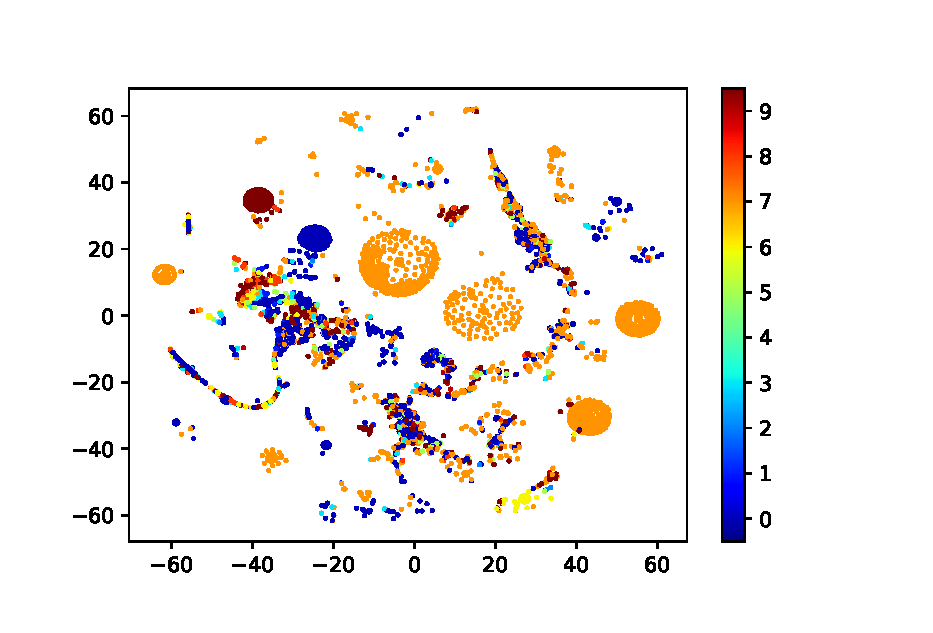
\includegraphics[width=0.6\textwidth]{../.././Data/Figures/tsne.eps}\\
		\caption{T-SNE}\label{fig:tsne}
	\end{figure}
	
\end{slide}
%%
%%==========================================================================================

%%==========================================================================================
%%
\begin{slide}{PCA}
The PCA method using maximum likelihood estimation can only be reduced to 798 dimensions. The image below is a visualization image reduced to 2 dimensions using PCA.
\bigskip
\begin{figure}
	\centering
	\selectcolormodel{rgb}
	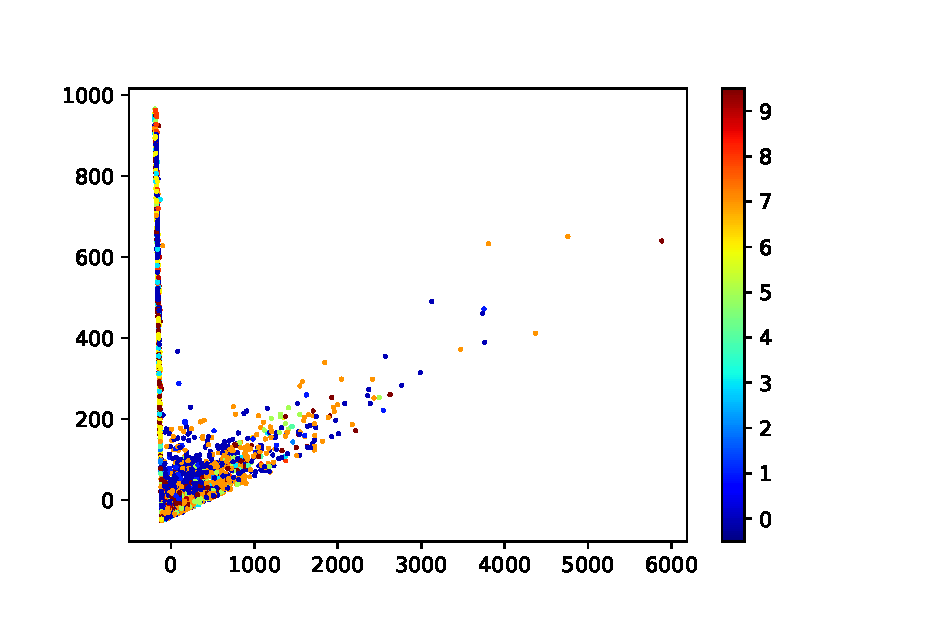
\includegraphics[width=0.6\textwidth]{../.././Data/Figures/pca.eps}\\
	\caption{pca-2D}\label{fig:pca-2D}
\end{figure}

\end{slide}
%%
%%==========================================================================================

\section{One-Class Classification}

%%==========================================================================================
%%
\begin{slide}{One-Class SVM}
\begin{figure}
	\centering
	\selectcolormodel{rgb}
	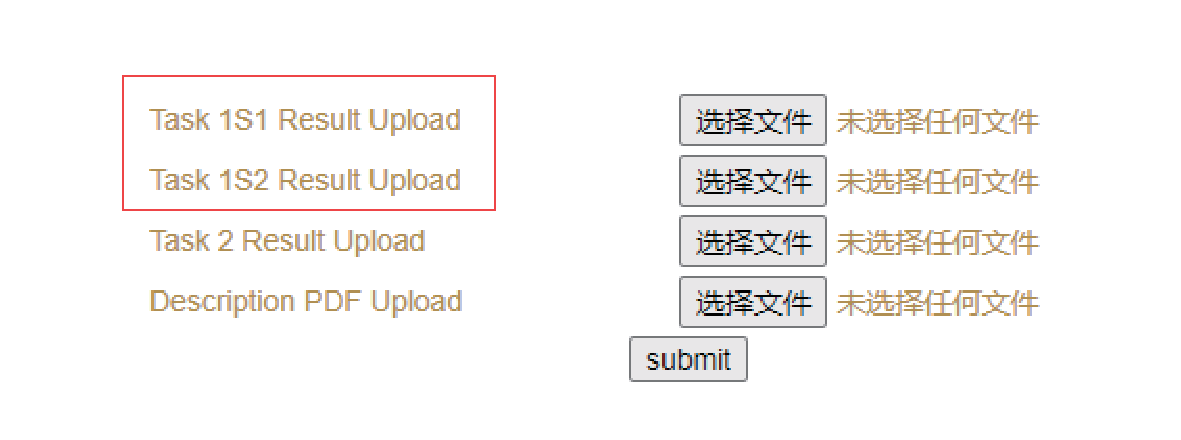
\includegraphics[width=0.6\textwidth]{../.././Data/Figures/tmp.eps}\\
	\label{fig:tmp}
\end{figure}
\end{slide}
%%
%%==========================================================================================

%%==========================================================================================
%%
\begin{slide}{Variational Auto-Encoder}
\begin{itemize}
	\item \textcolor{orange}{Hierarchial VAE}
	\item \textcolor{orange}{Other models?}
\end{itemize}
\end{slide}
%%
%%==========================================================================================

%%==========================================================================================
% TODO: Contact Page
\begin{wideslide}[toc=,bm=]{End}
\centering
\vspace{\stretch{1}}
\twocolumn[
lcolwidth=0.35\linewidth,
rcolwidth=0.65\linewidth
]
{
% \centerline{
\includegraphics[scale=.2]{tulip-logo.eps}}
}
{
\vspace{\stretch{1}}
Thank you!
}
\vspace{\stretch{1}}
\end{wideslide}

\end{document}

\endinput
